\chapter{Analisi del contesto aziendale}
	\section{L'azienda e il suo ambito di attività}
		PastBook è una piccola azienda con sede ad Amsterdam, nei Paesi Bassi. Essa offre agli utenti la possibilità di creare e stampare
		degli album fotografici personalizzati.
		\begin{figure}[H]
			\centering
			
\includegraphics[width=0.4\textwidth]{capitolo_1/immagini/logo_pastbook.png}
			\caption[Logo di PastBook]{Logo di PastBook\protect\footnotemark}
		\end{figure}
		\footnotetext{Immagine tratta da \url{https://fronteers.nl/_img/werkgevers/pastbook.png}}
		\noindent Il progetto nasce nel 2012 quando Stefano Cutello — fondatore e attuale titolare di PastBook — decide di abbandonare il
		posto di lavoro presso eBay\footnote{\url{http://www.ebay.com}} per realizzare la propria idea. L'esigenza è riscoprire i
		ricordi pubblicati ogni giorno sui social network: infatti, le vite delle persone sono ormai completamente online e non esiste più
		niente di stampato.\\
		L'azienda descrive il servizio che essa offre nel seguente modo:
		\hyphenblockquote{english}{Many things can disappear — not your memories. We believe that certain moments can last forever. We
			believe that the best things in the world are not things. We help you rediscover your memories. We collect the highlights of
			your life moments and provide you with a tangible way to relive them — in PastBook.}
		PastBook, dunque, aiuta le persone a raccogliere le proprie foto sparse per il Web e permette loro di creare un album fotografico
		che memorizzi in modo permanente i ricordi più belli.
	\section{Prodotti offerti}
		\subsection{Photo Books in un click}
			Esistono varie aziende che permettono agli utenti di creare album fotografici a partire dalle immagini presenti nei social
			network. PastBook differisce da esse per un importante principio che sta alla base della realizzazione del prodotto: l'utente
			deve poter creare il proprio Photo Book in modo veloce ed automatico, senza pensare a particolari che distolgano la sua mente
			dallo scopo.\\
			L'azienda prevede che i propri clienti debbano solo scegliere il servizio dal quale intendono ottenere le immagini. Il resto
			è automatico: non è previsto che l'utente abbia la possibilità di personalizzare il proprio Photo Book durante la sua
			realizzazione. I più esigenti possono fare piccole modifiche solo a creazione avvenuta.\\
			\begin{multicols}{3}[\noindent PastBook permette di recuperare le immagini utilizzando uno dei seguenti servizi Web:]
				\begin{itemize}
					\item Instagram\footnote{\url{http://www.instagram.com}}

					\item Facebook\footnote{\url{http://www.facebook.com}}

					\item Flickr\footnote{\url{http://www.flickr.com}}

					\item Google Drive\footnote{\url{http://www.google.com/drive}}

					\item Dropbox\footnote{\url{http://www.dropbox.com}}

					\item OneDrive\footnote{\url{http://onedrive.live.com}}

					\item Picasa\footnote{\url{http://picasa.google.com}}

					\item Evernote\footnote{\url{http://www.evernote.com}}

					\item Box\footnote{\url{http://www.box.com}}

				\end{itemize}
			\end{multicols}
			\begin{figure}[H]
				\centering
				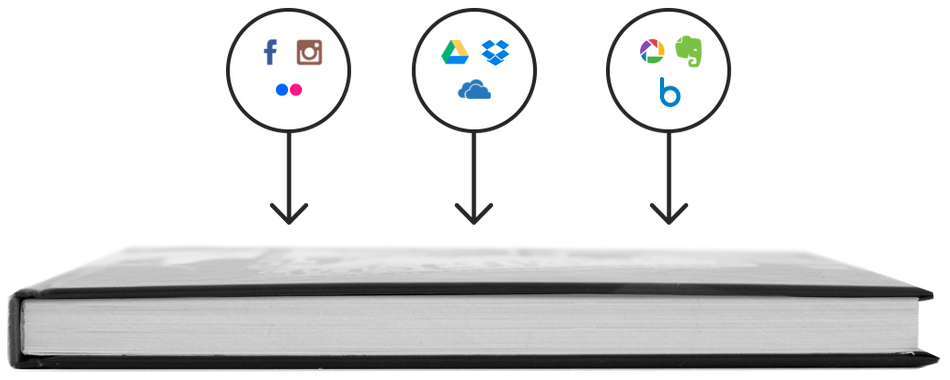
\includegraphics[width=0.9\textwidth]{capitolo_1/immagini/photo_book_one_click.png}
				\caption[Photo Book in un click]{Photo Book in un click\protect\footnotemark}
			\end{figure}
			\footnotetext{Immagine tratta da \url{https://www.pastbook.com/beautiful-photo-books/}}
			\noindent Gli utenti hanno inoltre la possibilità di invitare chiunque ad aggiungere ulteriori ricordi al proprio Photo Book,
			condividendo un link privato tramite email, QR code, Facebook o Twitter\footnote{\url{http://www.twitter.com}}.
		\subsection{Photo Books personalizzati}
			PastBook offre anche una seconda tipologia di prodotti: Photo Book creati su misura da designer professionisti. Tale offerta
			è rivolta ai clienti che non pretendono risultati immediati ma che allo stesso tempo esigono una qualità superiore.
			\begin{figure}[H]
				\centering
				
\includegraphics[width=0.9\textwidth]{capitolo_1/immagini/photo_book_personalizzato.png}
				\caption[Realizzazione di un Photo Book personalizzato]{Realizzazione di un Photo Book personalizzato\protect\footnotemark}
			\end{figure}
			\footnotetext{Immagine tratta da \url{https://www.pastbook.com/elite/}}
			\noindent Gli utenti, in particolare, dopo aver mandato le proprie foto, possono interagire direttamente con la persona che
			si sta occupando della creazione del Photo Book per indicare le immagini preferite o per esprimere eventuali preferenze
			riguardanti lo stile, i testi, i colori, etc.
	\section{Organizzazione aziendale}
		\subsection{Obiettivi e risultati attesi}
			PastBook persegue obiettivi di tre tipologie differenti:
			\begin{itemize}
				\item tecnici, legati al funzionamento dei prodotti;
				\item economici, legati alla produttività, all'efficacia e all'efficienza;
				\item sociali, legati alla qualità della vita e in particolare alla qualità della vita di lavoro.
			\end{itemize}
			\subsubsection{Qualità del prodotto e dei processi}
				Il principale obiettivo di PastBook è realizzare un algoritmo che sia in grado di produrre in modo
				automatico un Photo Book che sia conforme alle aspettative dei clienti. Oltre a ciò, l'azienda intende raggiungere
				precisi traguardi riguardanti l'efficienza del processo di creazione del prodotto: esso deve avvenire nel minor tempo
				possibile e impiegando una quantità minima di risorse.\\
				Questi obiettivi puramente tecnici celano lo scopo economico di riuscire a vendere i Photo Book realizzati in modo
				automatico ad un prezzo inferiore rispetto a quello proposto della concorrenza, pur mantenendo elevata la
				soddisfazione dei clienti.
			\subsubsection{Semplicità di utilizzo degli strumenti}
				PastBook sposa da sempre una precisa filosofia: gli strumenti a disposizione degli utenti devono essere semplici,
				per non dire basilari. In particolare, l'azienda vuole che il cliente riesca ad ottenere qualcosa di gradito — non
				per forza perfetto — senza sentire il bisogno di dover intervenire per apportare modifiche.\\
				L'uso di questo tipo di approccio si basa sulle seguenti considerazioni:
				\begin{itemize}
					\item Spesso gli utenti provano un nuovo servizio per pura curiosità e, di conseguenza, non sono disposti ad
					utilizzare molto del proprio tempo per giungere al risultato. Numerose possibilità di modifiche e
					personalizzazioni non farebbero altro che spazientire l'utente. Un'azienda deve dunque saper sfruttare il
					breve contatto con il potenziale cliente per poterlo conquistare
					\item Quanto più è il tempo a disposizione di un utente per valutare un acquisto in modo razionale tanto
					meno influiscono su di esso impulsi ed emozioni. È dunque necessario saper cogliere l'irrazionalità iniziale
					del cliente per persuaderlo: per ottenere ciò, la quantità di azioni svolta per creare un Photo Book deve
					essere minima.
				\end{itemize}
			\subsubsection{Valorizzazione del capitale umano}
				Il titolare di PastBook è fermamente convinto che una forte cultura organizzativa sia un fattore critico per le
				performance e il successo dell'azienda. Egli, in particolare, cerca continuamente di motivare e coinvolgere i propri
				dipendenti per fare in modo che essi apprezzino i risultati che il loro lavoro può portare.\\
				In aggiunta, PastBook crede fortemente al fatto che la produttività del personale sia influenzata dalla qualità dei
				rapporti che si instaurano tra le persone facenti parte del team: ciascuno, con le proprie motivazioni, influenza
				positivamente gli altri individui del gruppo, facilitando il raggiungimento dei risultati imposti.\\
				\begin{figure}[H]
	\centering
	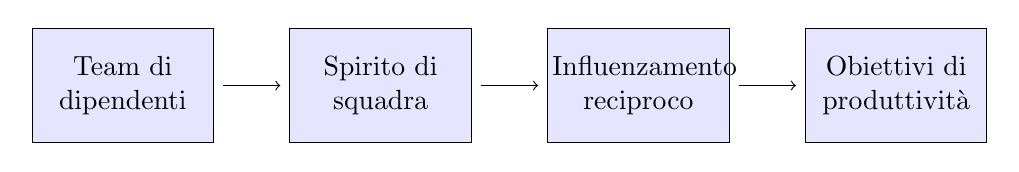
\begin{tikzpicture}
		\draw[fill=blue,fill opacity=0.1] (0,0) rectangle ++(0.19\textwidth,0.12\textwidth);
		\draw (0,0) rectangle ++(0.19\textwidth,0.12\textwidth)
		node[pos=.5, text width=0.18\textwidth, align=center] {Team di dipendenti};
		\draw[->] (0.20\textwidth,0.06\textwidth) -- (0.26\textwidth,0.06\textwidth);
		\draw[fill=blue,fill opacity=0.1] (0.27\textwidth,0) rectangle ++(0.19\textwidth,0.12\textwidth);
		\draw (0.27\textwidth,0) rectangle ++(0.19\textwidth,0.12\textwidth)
		node[pos=.5, text width=0.18\textwidth, align=center] {Spirito di squadra};
		\draw[->] (0.47\textwidth,0.06\textwidth) -- (0.53\textwidth,0.06\textwidth);
		\draw[fill=blue,fill opacity=0.1] (0.54\textwidth,0) rectangle ++(0.19\textwidth,0.12\textwidth);
		\draw (0.54\textwidth,0) rectangle ++(0.19\textwidth,0.12\textwidth)
		node[pos=.5, text width=0.18\textwidth, align=center] {Influenzamento reciproco};
		\draw[->] (0.74\textwidth,0.06\textwidth) -- (0.80\textwidth,0.06\textwidth);
		\draw[fill=blue,fill opacity=0.1] (0.81\textwidth,0) rectangle ++(0.19\textwidth,0.12\textwidth);
		\draw (0.54\textwidth,0) (0.81\textwidth,0) rectangle ++(0.19\textwidth,0.12\textwidth)
		node[pos=.5, text width=0.18\textwidth, align=center] {Obiettivi di produttività};
	\end{tikzpicture}
\end{figure}

				Infine, per fare in modo che ognuno esprima al meglio le proprie potenzialità, l'azienda intende decentralizzare le
				responsabilità ed aumentare l'autonomia decisionale. Parallelamente, ogni dipendente deve cercare di comprendere
				pienamente i limiti entro i quali può operare in modo autonomo.
		\subsection{Risorse disponibili}
			PastBook può avvalersi di numerose risorse per poter raggiungere gli obiettivi prefissati.\\
			Innanzitutto, l'azienda ha a disposizione i propri dipendenti e collaboratori: mentre alcuni di essi forniscono il proprio
			contributo solo per breve tempo, altri lavorano per PastBook in modo stabile. In particolare, durante il periodo in cui ho
			svolto lo stage, l'azienda era composta da 7-9 persone. In aggiunta, alcuni mentori che hanno contribuito a far crescere
			PastBook durante i suoi esordi offrono spesso il proprio aiuto per individuare le strategie vincenti.\\
			Per quanto riguarda le risorse economiche, l'azienda può fare affidamento su una serie di investitori privati che credono
			fortemente nel progetto e nelle persone che lo stanno realizzando. Essi forniscono perlopiù sostegno finanziario e non hanno
			ruoli di tipo decisionale.\\
			Le risorse tecnologiche necessarie all'azienda sono molto poche. Infatti, ogni persona lavora utilizzando il proprio PC e
			solo in casi particolari utilizza dispositivi di altro tipo.\\
			Per quanto riguarda gli spazi, infine, i dipendenti di PastBook possono usufruire, oltre che dell'ufficio, anche di due
			cucine e di una sala relax.
		\subsection{Componenti e relazioni organizzative}
			\subsubsection{Funzioni e ruoli}
				In PastBook le responsabilità di ciascuna persona sono ben definite. Questo aiuta i dipendenti a capire i propri
				confini operativi e a diminuire le dimenticanze.\\
				L'azienda — per funzionare in modo corretto — necessita dei seguenti ruoli:
				\begin{center}
					\rowcolors{1}{azzurro_chiaro}{azzurro}
					\begin{tabular}[H]{p{0.25\textwidth} p{0.60\textwidth}}
						Dirigente 			& Si occupa della gestione delle risorse disponibili e del
										  coordinamento generale per poter raggiungere gli obiettivi
										  prefissati.\\
						\hline
						Responsabile finanziario	& Si occupa della gestione e della supervisione delle attività
										  finanziarie.\\
						\hline
						Responsabile del marketing	& Si occupa della comunicazione sui social media, attuando strategie
										  per aumentare il valore percepito dai consumatori rispetto al
										  prodotto offerto.\\
						\hline
						Customer relationship manager	& Si occupa della gestione delle relazioni con i clienti. Questo
										  implica un approccio operativo (risposte tempestive ed efficaci
										  alle richieste) e uno analitico (analisi dei bisogni e della
										  soddisfazione per sviluppare un'offerta commerciale appropriata).\\
						\hline
						Grafico				& Fornisce supporto e consulenza artistica durante la progettazione
										  dei vari prodotti (sito web, applicazioni mobile, banner
										  pubblicitari, etc.).\\
						\hline
						Chief technical officer		& Supervisiona l'implementazione dei prodotti e dei servizi offerti
										  per assicurare che portino valore aggiunto all'azienda. Coglie le
										  potenzialità di nuove tecnologie per convertirle in decisioni
										  strategiche per l'azienda.\\
						\hline
						Sviluppatore 			& Si occupa dei vari aspetti del ciclo di vita di un prodotto
										  software.\\
					\end{tabular}
				\end{center}
				Alcuni dipendenti aziendali, a seconda delle necessità, possono ricoprire più di una mansione.
			\subsubsection{Struttura organizzativa}
				L'azienda è suddivisa in tre unità organizzative, individuate sulla base degli obiettivi che ognuna di esse si impone
				di raggiungere:
				\begin{itemize}
					\item all'\emph{area amministrativa}, che si occupa di aspetti economici e decisionali, appartengono il
					dirigente e il responsabile finanziario;
					\item all'\emph{area commerciale}, che si occupa delle strategie di mercato, della commercializzazione del
					prodotto e dell'assistenza ai clienti, appartengono tutti i membri del front office e il responsabile del
					marketing;
					\item all'\emph{area ricerca e sviluppo}, che studia come migliorare i prodotti o come crearne di nuovi,
					appartengono il CTO, gli sviluppatori e il grafico.
				\end{itemize}
				\begin{figure}[H]
	\centering
	\begin{tikzpicture}
		\draw[fill=azzurro] (0,0) rectangle ++(0.20\textwidth,0.12\textwidth);
		\draw (0,0) rectangle ++(0.20\textwidth,0.12\textwidth)
		node[pos=.5, text width=0.18\textwidth, align=center] {Area commerciale};
		\draw[fill=azzurro] (0.56\textwidth,0) rectangle ++(0.20\textwidth,0.12\textwidth);
		\draw (0.56\textwidth,0) rectangle ++(0.20\textwidth,0.12\textwidth)
		node[pos=.5, text width=0.18\textwidth, align=center] {Area ricerca e sviluppo};
		\draw[fill=azzurro] (0.28\textwidth,0.13\textwidth) rectangle ++(0.20\textwidth,0.12\textwidth);
		\draw (0.28\textwidth,0.13\textwidth) rectangle ++(0.20\textwidth,0.12\textwidth)
		node[pos=.5, text width=0.18\textwidth, align=center] {Area amministrativa};
		\draw (0.21\textwidth,0.06\textwidth) -- (0.55\textwidth,0.06\textwidth);
		\draw (0.38\textwidth,0.06\textwidth) -- (0.38\textwidth,0.12\textwidth);
	\end{tikzpicture}
\end{figure}

				PastBook, essendo una realtà aziendale molto piccola, non prevede la presenza di organi di comando e relativi
				subordinati. Tuttavia, per ognuna delle unità organizzative è possibile individuare una persona che funge da
				riferimento per i colleghi: una sorta di leader informale, che trae la sua legittimazione dal consenso degli altri
				membri.\\
				Molto spesso — per far fronte a nuovi problemi o per tentare di raggiungere specifici obiettivi — persone provenienti
				da unità diverse formano dei gruppi di lavoro temporanei, non descrivibili all'interno dell'organigramma. Questi
				gruppi sono formati per sfruttare competenze in ambiti diversi e per affrontare i problemi da diversi punti di vista.
				Accade spesso, per esempio, che gli esperti di marketing collaborino con i membri dell'area ricerca e sviluppo per
				poter realizzare un prodotto di valore sia dal punto di vista funzionale che commerciale.
			\subsubsection{Coordinamento e controllo}
				Stefano Cutello — attuale dirigente di PastBook — ha un duplice compito: gestire le attività correnti dell'azienda e
				contemporaneamente cercare nuove opportunità, prevedendo i mutamenti e sviluppando una strategia interna attraverso
				la conoscenza del contesto esterno. Oltre che manager, egli è anche il leader effettivo del team: ha la capacità di
				comunicare, di interagire, di gestire le relazioni. In particolare, egli motiva costantemente i suoi collaboratori a
				dare il meglio di sé per poter raggiungere gli obiettivi prefissati.\\
				Per controllare e coordinare il flusso delle attività in azienda, Stefano ha scelto di applicare una tecnica molto
				simile allo Scrum\footnote{\url{http://www.scrum.org} Framework agile per lo sviluppo del software, concepito per gestire progetti e prodotti. I cicli di feedback
ne costituiscono le tecniche di gestione fondamentali.}. Ogni mattina, prima di cominciare a lavorare, avviene il
				cosiddetto \emph{daily standup}, un breve incontro durante il quale ogni membro del team prende la parola per pochi
				minuti e spiega agli altri due cose:
				\begin{itemize}
					\item che attività ha svolto il giorno precedente precedente e quali risultati ha ottenuto (gli obiettivi
					fissati sono stati raggiunti?);
					\item cosa intende fare il giorno stesso e quali risultati vuole ottenere (quali obiettivi si pone?).
				\end{itemize}
				Durante il meeting giornaliero ognuno è anche invitato a condividere dubbi, ostacoli o impedimenti emersi durante le
				proprie attività: in questo modo è possibile ricevere consigli o aiuto diretto da parte dei colleghi.\\
				Per controllare il lavoro di ciascuno, inoltre, il dirigente utilizza
				\emph{Trello}\footnote{\url{http://www.trello.com} Applicazione web che permette di rappresentare un progetto tramite una \emph{board} che contiene alcune
\emph{lists} (corrispondenti a liste di task). Ogni list contiene delle \emph{cards} (corrispondenti a task). Le card possono essere spostate da una
lista alla successiva, tramite un semplice \emph{drag-and-drop}.}. Nello specifico, ogni dipendente ha accesso alle board riguardanti
				i progetti ai quali collabora. Ogni board è composta da tre liste: \emph{TODO} (contenente ciò che non è ancora
				stato fatto), \emph{DOING} (che contiene informazioni riguardanti quanto è in corso d'opera) e \emph{DONE} (un
				elenco dei task portati a termine). Ogni membro di una certo progetto deve preoccuparsi di mantenere aggiornate le
				posizioni delle card a lui assegnate all'interno della board. In questo modo il dirigente o il responsabile di un
				progetto è sempre in grado di capire quanto manchi al raggiungimento degli obiettivi prefissati.\\
				Per permettere un coordinamento più generale, oltre ai brevi incontri giornalieri in azienda sono previste riunioni
				con cadenza mensile alle quali tutti i membri del team sono invitati a partecipare tramite il proprio contributo.
				Questi meeting sono più impegnativi rispetto ai daily standup (durano fino a quattro ore) e includono i seguenti
				elementi:
				\begin{itemize}
					\item Ogni unità organizzativa riassume quanto è avvenuto durante il mese trascorso, con particolare
					riferimento all'eventuale raggiungimento degli obiettivi fissati. In particolare, l'area amministrativa
					riporta i dati riguardanti la situazione finanziaria, l'area commerciale si concentra sull'uso che la
					clientela fa dei servizi e sul funzionamento delle campagne pubblicitarie, l'area ricerca e sviluppo mostra
					i progressi fatti nella realizzazione di nuovi prodotti.
					\item Ogni membro del team esamina e commenta i dati riportati dalle varie unità, identificando cosa è andato
					bene e cosa possa essere potenzialmente migliorato. Al termine di questa attività il team fissa obiettivi
					concreti da raggiungere nel mese seguente.
					\item Il dirigente pianifica il lavoro che deve essere svolto per poter raggiungere gli obiettivi fissati e
					delega le varie responsabilità. Eventualmente egli dispone che alcuni dipendenti formino dei gruppi di
					progetto per poter affrontare e risolvere dati problemi.
				\end{itemize}
			\subsubsection{Gestione del personale}
				Il personale è una dei fattori di successo di PastBook: i dipendenti sono molto coinvolti nei processi decisionali
				ed è richiesta loro una grande flessibilità nel ricoprire mansioni all'interno dell'azienda. Di conseguenza, il ruolo
				di chi si occupa del personale è fondamentale.\\
				La gestione delle risorse umane svolge prevalentemente le seguenti attività:
				\begin{itemize}
					\item selezionare e formare;
					\item motivare e coinvolgere.
				\end{itemize}
				Innanzitutto, l'efficienza e la potenzialità di PastBook dipendono in larga misura dall'attenta \emph{selezione} dei
				collaboratori: eventuali errori commessi in tale fase comportano conseguenze negative per l'azienda. Il processo
				selettivo comporta un'attenta analisi delle capacità, abilità e caratteristiche personali degli individui esaminati.
				In particolare, per l'azienda è importante che essi siano in larga misura indipendenti nel modo di lavorare e nel
				saper prendere decisioni ponderate e sensate nei momenti di difficoltà.\\
				In secondo luogo, l'azienda riconosce l'importanza della \emph{formazione} del personale: gli individui che sono
				stati inseriti nel team necessitano di un rapido potenziamento delle conoscenze e delle capacità per poter lavorare
				in autonomia quanto prima. L'obiettivo del processo formativo è raggiunto grazie all'attuazione di percorsi di
				affiancamento: essi permettono al nuovo membro del gruppo di capire sia il metodo di lavoro utilizzato a PastBook che
				le regole e i valori che non sono stati formalizzati.\\
				L'ultimo compito di coloro che gestiscono le risorse umane è \emph{motivare} e allo stesso tempo
				\emph{coinvolgere} il personale, facendo in modo che i dipendenti abbiano un atteggiamento mentale positivo nei
				confronti dei loro compiti e responsabilità. Per poter raggiungere questi obiettivi, il team è costantemente
				stimolato a cimentarsi in nuove esperienze e a proporre nuove idee. Inoltre, i legami di amicizia fra colleghi sono
				incoraggiati tramite attività terze da svolgere eventualmente anche durante l'orario di lavoro.
			\subsubsection{Gestione dei clienti}
				PastBook cerca costantemente di sviluppare un orientamento strategico che pone l'attenzione sulla costruzione e il
				mantenimento di una base di clienti fedeli che siano in grado di incrementare la redditività nel medio-lungo
				termine.\\
				L'enfasi posta sullo sviluppo nel tempo di relazioni con la clientela — piuttosto che soltanto sulla chiusura di una
				singola transazione di vendita — comporta numerosi vantaggi. Innanzitutto, i ricavi incrementano grazie a una
				riduzione dei costi, dovuta soprattutto a un mercato nel quale si gioca a sottrarre clienti alla concorrenza tramite
				azioni promozionali aggressive rivolte ai nuovi utenti. In secondo luogo, l'azienda può contare su un flusso costante
				di entrate. Inoltre, clienti fedeli (e dunque soddisfatti) danno spesso origine a un passaparola che, se assume una
				consistenza significativa, può contribuire notevolmente al miglioramento dell'immagine aziendale. Infine, un
				vantaggio di natura immateriale riguarda la possibilità di sviluppare più facilmente soluzioni innovative: i clienti,
				se correttamente coinvolti nel processo di miglioramento del prodotto, possono proporre idee che incrementino la
				competitività stessa dell'azienda.
				\begin{figure}[H]
	\centering
	\begin{tikzpicture}
		\draw[fill=azzurro] (0,0) rectangle ++(0.22\textwidth,0.12\textwidth);
		\draw (0,0) rectangle ++(0.22\textwidth,0.12\textwidth)
		node[pos=.5, text width=0.17\textwidth, align=center] {Minori costi di gestione};
		\draw[fill=azzurro] (0.26\textwidth,0) rectangle ++(0.22\textwidth,0.12\textwidth);
		\draw (0.26\textwidth,0) rectangle ++(0.22\textwidth,0.12\textwidth)
		node[pos=.5, text width=0.17\textwidth, align=center] {Flussi di entrate costanti};
		\draw[fill=azzurro] (0.52\textwidth,0) rectangle ++(0.22\textwidth,0.12\textwidth);
		\draw (0.52\textwidth,0) rectangle ++(0.22\textwidth,0.12\textwidth)
		node[pos=.5, text width=0.17\textwidth, align=center] {Passaparola positivo};
		\draw[fill=azzurro] (0.78\textwidth,0) rectangle ++(0.22\textwidth,0.12\textwidth);
		\draw (0.78\textwidth,0) rectangle ++(0.22\textwidth,0.12\textwidth)
		node[pos=.5, text width=0.17\textwidth, align=center] {Collaborazione con i clienti orientati all'innovazione};
		\draw (0.11\textwidth,0.19\textwidth) -- (0.89\textwidth,0.19\textwidth);
		\draw[->] (0.11\textwidth,0.19\textwidth) -- (0.11\textwidth,0.13\textwidth);
		\draw[->] (0.37\textwidth,0.19\textwidth) -- (0.37\textwidth,0.13\textwidth);
		\draw[->] (0.63\textwidth,0.19\textwidth) -- (0.63\textwidth,0.13\textwidth);
		\draw[->] (0.89\textwidth,0.19\textwidth) -- (0.89\textwidth,0.13\textwidth);
		\draw (0.50\textwidth,0.19\textwidth) -- (0.50\textwidth,0.25\textwidth);
		\draw[fill=azzurro_scuro] (0.39\textwidth,0.26\textwidth) rectangle ++(0.22\textwidth,0.12\textwidth);
		\draw (0.39\textwidth,0.26\textwidth) rectangle ++(0.22\textwidth,0.12\textwidth)
		node[pos=.5, text width=0.17\textwidth, align=center] {Cliente fedele};
	\end{tikzpicture}
\end{figure}

				Per aumentare la fedeltà e il grado di soddisfazione della clientela, l'area aziendale dedicata alle relazioni con
				i clienti svolge due attività:
				\begin{itemize}
					\item \emph{Assistenza personalizzata}, ovvero aiuto rivolto agli utenti che riscontrano problemi durante
					l'utilizzo dei prodotti offerti da PastBook. L'operatore aziendale, oltre a fornire le corrette	indicazioni
					richieste, si preoccupa di raccogliere dati che riguardano come il prodotto è percepito dal cliente. Questi
					dati sono poi rielaborati dall'amministrazione per cercare di pianificare e attuare strategie commerciali
					adatte.
					\item {Mantenimento di un blog} aziendale nel quale sono inseriti sia suggerimenti su come usare gli
					strumenti messi a disposizione da PastBook che fatti, eventi e curiosità che possono stuzzicare la mente del
					lettore. Il blog è innanzitutto lo strumento grazie al quale l'azienda suggerisce implicitamente delle
					occasioni durante le quali un cliente può pensare di realizzare e comprare un Photo Book. In secondo luogo il
					blog è il mezzo tramite cui il pubblico è informato delle novità introdotte e delle promozioni in corso.
				\end{itemize}
			\subsubsection{Comunicazione nell'azienda}
				I dipendenti aziendali comunicano tra loro prevalentemente tramite contatti informali, fortemente basati sulle
				relazioni. Non è presente alcun tipo di struttura gerarchica che preveda controlli sui modi di comunicare tra membri
				appartenenti ad aree differenti dell'azienda. Questo modo di comunicare è fortemente dovuto al fatto che tutto il
				personale lavori all'interno di una stessa grande stanza.\\
				Il principale strumento informatico di supporto alla comunicazione è \emph{Slack}\footnote{\url{http://www.slack.com} Strumento di collaborazione multi-piattaforma, ideale per i team di lavoro. Questo tool annovera le funzionalità
ormai “classiche” delle chat, tra le quali la possibilità di creare canali di comunicazione tematici, di riservare messaggi a determinati colleghi e
di condividere file. Inoltre, esso garantisce numerosi altri vantaggi a coloro che lo usano per lavorare in gruppo: collaborazione durante la modifica
di \emph{snippet} di codice, \emph{screen sharing} e comunicazione video. Il vero punto di forza, tuttavia, è rappresentato dalla possibilità di
integrazione con centinaia dei più importanti software presenti sul mercato (Twitter, Dropbox, GitHub, Heroku, Trello etc.).}:
				ogni unità organizzativa aziendale e ogni gruppo di progetto possiede un proprio canale nel quale possono essere
				ospitate conversazioni, scambiati file e condivise porzioni di codice.
	\section{Sviluppo software}
		\subsection{Metodologia di lavoro}
			\subsubsection{Tipico ciclo di vita del software}
				L'idea alla base di un prodotto software sviluppato da PastBook deriva molto spesso dal contributo portato
				dall'intero team durante i meeting mensili. Queste occasioni, infatti, danno l'opportunità ai dipendenti di esprimere
				la propria opinione con lo scopo di migliorare la qualità dei servizi e dei prodotti offerti dall'azienda. Quando il
				concetto proposto dimostra di poter essere di effettivo valore, il dirigente sceglie alcuni membri del team e li
				assegna a un gruppo di progetto dedicato.\\
				Il passo successivo nello sviluppo dell'idea consiste solitamente in una breve analisi dei requisiti, durante la
				quale il gruppo cerca di delineare le caratteristiche e i requisiti che il prodotto dovrà avere. Ogni membro del
				gruppo individua contemporaneamente quale sia la propria parte di lavoro e come questa possa successivamente
				integrarsi con le attività svolte dai colleghi.\\
				A questo punto, a seconda delle abilità e delle capacità presenti nel gruppo di lavoro, lo sviluppo del prodotto
				si divide parti in distinte:
				\begin{itemize}
					\item Gli sviluppatori sono sempre presenti. Essi sono eventualmente coordinati dal CTO. Il loro compito è
					di progettare e codificare in modo appropriato le varie funzionalità individuate durante l'attività di
					analisi.
					\item Se il prodotto è destinato al pubblico allora quasi sempre il grafico comincia a delineare
					l'interfaccia. Egli sta in stretto contatto con gli sviluppatori, aggiornandoli su eventuali requisiti
					che essi devono soddisfare.
					\item Molto spesso nella realizzazione del prodotto sono coinvolti dipendenti che hanno capacità commerciali.
					Essi svolgono prevalentemente funzioni di supporto a chi si occupa della grafica. Infatti, danno indicazioni
					sui metodi migliori per interagire con la clientela e per intrattenerla e coinvolgerla allo stesso tempo.
				\end{itemize}
				Obiettivo primario di qualsiasi gruppo di progetto software all'interno di PastBook è sempre mettere a
				disposizione del resto dell'azienda un prototipo funzionante nel minor tempo possibile: in questo modo il prodotto può
				essere testato dall'intero team. Infine, quando il prototipo raggiunge una maturità sufficiente, esso è distribuito
				anche ad utenti esterni a PastBook, in modo tale che ne possano testare le funzionalità.\\
				Dopo il rilascio del prodotto, il gruppo di progetto si scioglie. Quando insorgono problemi e si rende necessaria
				attività di manutenzione, il dirigente delega la responsabilità a un dipendente adatto alla mansione.
				\begin{figure}[H]
	\centering
	\begin{tikzpicture}
		\draw[fill=azzurro] (0,0.60\textwidth) rectangle ++(0.24\textwidth,0.10\textwidth);
		\draw (0,0.60\textwidth) rectangle ++(0.24\textwidth,0.10\textwidth)
		node[pos=.5, text width=0.22\textwidth, align=center] {Concepimento idea e formazione dei gruppo di lavoro};
		
		\draw (0.25\textwidth,0.65\textwidth) -- (0.28\textwidth,0.65\textwidth);
		\draw[->] (0.28\textwidth,0.65\textwidth) -- (0.28\textwidth,0.59\textwidth);
		
		\draw[fill=azzurro] (0.16\textwidth,0.48\textwidth) rectangle ++(0.24\textwidth,0.10\textwidth);
		\draw (0.16\textwidth,0.48\textwidth) rectangle ++(0.24\textwidth,0.10\textwidth)
		node[pos=.5, text width=0.22\textwidth, align=center] {Analisi dei requisiti};
		
		\draw (0.41\textwidth,0.53\textwidth) -- (0.44\textwidth,0.53\textwidth);
		\draw[->] (0.44\textwidth,0.53\textwidth) -- (0.44\textwidth,0.47\textwidth);
		
		\draw (0.31\textwidth,0.12\textwidth) rectangle ++(0.26\textwidth,0.34\textwidth);
		
		\draw[fill=azzurro] (0.32\textwidth,0.35\textwidth) rectangle ++(0.24\textwidth,0.10\textwidth);
		\draw (0.32\textwidth,0.35\textwidth) rectangle ++(0.24\textwidth,0.10\textwidth)
		node[pos=.5, text width=0.22\textwidth, align=center] {Progettazione del software e codifica};
		
		\draw[fill=azzurro] (0.32\textwidth,0.24\textwidth) rectangle ++(0.24\textwidth,0.10\textwidth);
		\draw (0.32\textwidth,0.24\textwidth) rectangle ++(0.24\textwidth,0.10\textwidth)
		node[pos=.5, text width=0.22\textwidth, align=center] {Ideazione interfaccia grafica};
		
		\draw[fill=azzurro] (0.32\textwidth,0.13\textwidth) rectangle ++(0.24\textwidth,0.10\textwidth);
		\draw (0.32\textwidth,0.13\textwidth) rectangle ++(0.24\textwidth,0.10\textwidth)
		node[pos=.5, text width=0.22\textwidth, align=center] {Analisi del bisogno dei clienti};
		
		\draw (0.50\textwidth,0.47\textwidth) -- (0.50\textwidth,0.50\textwidth);
		\draw[->] (0.50\textwidth,0.50\textwidth) -- (0.69\textwidth,0.50\textwidth);
		
		\draw[dashed] (0.59\textwidth,0.50\textwidth) -- (0.55\textwidth,0.55\textwidth);
		\draw (0.47\textwidth,0.55\textwidth) rectangle ++(0.16\textwidth,0.08\textwidth)
		node[pos=.5, text width=0.16\textwidth, align=center] {Realizzazione prototipo};
		
		\draw (0.82\textwidth,0.44\textwidth) -- (0.82\textwidth,0.41\textwidth);
		\draw[->] (0.82\textwidth,0.41\textwidth) -- (0.58\textwidth,0.41\textwidth);
		
		\draw[dashed] (0.70\textwidth,0.41\textwidth) -- (0.75\textwidth,0.36\textwidth);
		\draw (0.67\textwidth,0.28\textwidth) rectangle ++(0.16\textwidth,0.08\textwidth)
		node[pos=.5, text width=0.16\textwidth, align=center] {Resoconti dei problemi};
		
		\draw[fill=azzurro] (0.70\textwidth,0.45\textwidth) rectangle ++(0.24\textwidth,0.10\textwidth);
		\draw (0.70\textwidth,0.45\textwidth) rectangle ++(0.24\textwidth,0.10\textwidth)
		node[pos=.5, text width=0.22\textwidth, align=center] {Collaudo};
		
		\draw (0.58\textwidth,0.29\textwidth) -- (0.61\textwidth,0.29\textwidth);
		\draw[->] (0.61\textwidth,0.29\textwidth) -- (0.61\textwidth,0.11\textwidth);
		
		\draw[fill=azzurro] (0.49\textwidth,0) rectangle ++(0.24\textwidth,0.10\textwidth);
		\draw (0.49\textwidth,0) rectangle ++(0.24\textwidth,0.10\textwidth)
		node[pos=.5, text width=0.22\textwidth, align=center] {Rilascio del prodotto};
	\end{tikzpicture}
	\caption{Ciclo di vita del software}
\end{figure}

			\subsubsection{Analisi dei requisiti}
				I gruppi di lavoro svolgono l'analisi dei requisiti durante le prime fasi di un progetto. In generale, il compito di
				tale attività è chiarire e dettagliare le caratteristiche e le funzioni che deve possedere il prodotto
				finale.\\
				Le direttive aziendali non prevedono che i dipendenti che svolgono questi compiti dedichino parte del loro tempo alla
				produzione di una documentazione formale. Dunque, i dati raccolti durante attività quali la definizione del
				problema, l'analisi di fattibilità e l'analisi del dominio non sono in alcun modo memorizzati in modo persistente.
				Non esiste nemmeno una vero e proprio documento che contenga la specifica dei requisiti. Infatti, i membri del
				gruppo di lavoro si limitano a utilizzare appunti, diagrammi e disegni fatti a mano: un incaricato, in seguito, si
				occupa della loro digitalizzazione e memorizzazione, senza però seguire alcun tipo di norma esplicita.\\
				Questo modo di procedere informale e talvolta impreciso ha diverse conseguenze negative. Innanzitutto, i requisiti
				sono  talvolta soggetti a interpretazione. In secondo luogo, essi possono mutare spesso durante le fasi successive
				dello sviluppo del prodotto.
			\subsubsection{Progettazione e codifica}
				La progettazione — intesa come attività che entra nel merito della struttura del sistema software, definendo come i
				requisiti devono essere soddisfatti — è un'esclusiva degli sviluppatori e del CTO.\\
				Tale attività intermedia tra analisi dei requisiti e codifica trova pochissimo spazio all'interno del ciclo di vita
				del software: l'obiettivo principale dell'azienda è poter ottenere un prototipo che funzioni quanto prima e la
				progettazione è ritenuta un formalismo che fa perdere tempo prezioso. Di conseguenza, non esiste alcun tipo di
				documentazione formale o informale che descrivi l'architettura del sistema e come essa si scomponga in moduli.\\
				Gli sviluppatori, piuttosto, devono essere esperti al punto tale da avere fin dall'inizio un'idea abbastanza precisa
				della struttura finale del sistema. La codifica, dunque, rappresenta l'attività predominante durante l'intero
				processo di sviluppo, poiché include in modo implicito molti dei compiti che dovrebbero essere assegnati a dei
				progettisti.\\
				PastBook è a conoscenza del fatto che questo approccio è molto rischioso nel medio e lungo termine: cambiamenti
				nell'architettura di un sistema software durante uno stato avanzato della produzione possono implicare ingenti
				perdite di energie, tempo e denaro. Tuttavia, l'azienda non vuole rinunciare al vantaggio di poter ottenere fin dalle
				fasi iniziali un prototipo funzionante del prodotto. Dunque, per evitare che errori gravi rischino di bloccare la
				realizzazione del prodotto, il dirigente di PastBook invita spesso gli sviluppatori a svolgere sessioni di
				\emph{pair programming}: queste permettono un confronto diretto sul campo per poter individuare le maggiori
				criticità.\\
				Per concludere, i programmatori si preoccupano costantemente di mantenere il codice sorgente ben strutturato e
				commentato, essendo esso l'unica forma di documentazione dalla quale trarre informazioni riguardanti il sistema
				software in questione. Anche il controllo di versione e la descrizione delle modifiche apportate di volta in volta
				sono eseguiti con particolare cura.
			\subsubsection{Collaudo}
				Tale attività serve per individuare le carenze di correttezza, completezza e affidabilità delle componenti software
				in corso di sviluppo.\\
				L'azienda prevede che per ogni prodotto siano eseguiti degli \emph{alpha test}: in pratica, il personale di PastBook
				sottopone il software a collaudo prima di procedere alla distribuzione al pubblico. Questi test — anche se non sono
				solitamente formalizzati e preparati a priori — sono molto specifici e coprono una parte significativa dei possibili
				casi d'uso. I programmatori, inoltre, prima di sottoporre il software a questo tipo di collaudo, arricchiscono il
				codice con istruzioni di controllo a runtime che facilitino il rilevamento degli errori.\\
				Il gruppo di lavoro, infine, distribuisce a individui esterni all'azienda alcuni prototipi che risultino abbastanza
				stabili e che abbiano superato con successo i test interni. Tali utenti eseguono i cosiddetti \emph{beta test}. In
				questo modo PastBook raggiunge due obiettivi:
				\begin{itemize}
					\item Utenti selezionati possono provare in anteprima i prodotti aziendali. Queste persone sono normalmente
					giornalisti o blogger che desiderano svelare in anteprima le funzionalità di un nuovo prodotto. L'azienda ha
					così la possibilità di pubblicizzare il proprio marchio. Talvolta i prodotti sono consegnati anche a
					possibili investitori che possono valutare le potenzialità di PastBook.
					\item Gli utenti usano il software in casi realistici e inviano al produttore resoconti dei malfunzionamenti
					riscontrati. Il gruppo di lavoro raccoglie in modo minuzioso i dati provenienti dai beta test per poi
					utilizzarli nell'individuazione e correzione di eventuali errori.
				\end{itemize}
				Ovviamente, gli sviluppatori sfruttano gli utenti esterni solo per testare i prodotti che sono pensati per il
				pubblico. Il software necessario al funzionamento interno di PastBook non viene reso noto al di fuori dei confini
				dell'azienda.
		\subsection{Tecnologie, tecniche e strumenti utilizzati}
			\subsubsection{Generazione di un Photo Book}
				L'azienda ha trovato un modo semplice ed efficace di generare i Photo Book, utilizzando in gran parte una tecnologia
				stabile ed affermata: \emph{WebKit}\footnote{Motore di rendering per pagine web. Al giorno d'oggi, alcuni dei principali browser sul mercato (quali Google Chrome, Opera e Safari) si
basano su di esso.}. In particolare, l'algoritmo sviluppato da
				PastBook non fa altro che utilizzare la funzione che converte una pagina composta da codice HTML e CSS in un
				documento PDF: la stessa che browser come Google Chrome\footnote{\url{http://www.google.com/chrome}} utilizzano per dare
				all'utente la possibilità di esportare i contenuti web nel formato sviluppato da Adobe Systems.\\
				L'utilizzo automatizzato di tale tecnologia è possibile grazie ai cosiddetti
				\emph{headless browser}\footnote{Web browser senza interfaccia grafica, eseguibile da linea di comando.} . PastBook, per esempio, fa uso di Google Chrome
				e delle API del suo motore di rendering che sono messe a disposizione degli sviluppatori.\\
				Il problema risulta dunque semplificato: ciò che il software aziendale deve fare è creare dinamicamente una
				rappresentazione formale del documento, senza preoccuparsi del suo successivo rendering. In particolare, l'algoritmo
				definisce innanzitutto la struttura dell'album tramite l'uso del linguaggio HTML e utilizzando le foto messe a
				disposizione dall'utente. In secondo luogo, aggiunge un foglio di stile CSS per formattare il contenuto
				precedentemente creato. WebKit porta a termine il resto del lavoro, generando il documento PDF a partire dai dati
				prodotti dal software PastBook.\\
				L'algoritmo dell'azienda è complesso non tanto nel rendering dell'album quanto nella creazione di una struttura e di
				una formattazione appropriata. Infatti, esso si occupa di disporre le immagini fornite in un modo che risulti
				gradevole all'utente. Inoltre, esso tenta di capire quali sono le foto migliori — qualsiasi cosa questo voglia dire —
				e quale di queste può essere scelta come copertina del Photo Book. L'algoritmo, allo stesso tempo, deve essere molto
				veloce, poiché gli utenti pretendono risultati istantanei.
			\subsubsection{API e Service}
				L'infrastruttura dei server di PastBook si base su due concetti fondamentali: \emph{API} e \emph{Service}.\\
				Il primo di questi concetti risponde esattamente alla definizione di web API che fornisce la letteratura:
				un'interfaccia di programmazione per un server web che è accessibile attraverso un endpoint e che permette a chi la
				usa di espletare un determinato compito. In particolare, le API aziendali mettono a disposizione degli sviluppatori
				le funzionalità basilari di cui essi hanno bisogno. Alcuni esempi sono:
				\begin{itemize}
					\item autenticazione al server PastBook
					\item creazione di un Photo Book vuoto
					\item aggiunta di una foto ad un Photo Book
					\item sostituzione della cover di un Photo Book
				\end{itemize}
				Le API hanno accesso diretto al database MySQL dell'azienda. Esse, inoltre, sono soggette a
				\emph{load balancing}\footnote{Tecnica informatica utilizzata nell'ambito dei sistemi informatici che consiste nel distribuire il carico di elaborazione di uno specifico
servizio tra più server.}, che permette maggiori livelli di scalabilità e
				affidabilità dell'intera architettura. Infatti, per gestire una grande quantità di utenti PastBook ha previsto più
				server identici tra di loro che possano prendersi carico delle richieste in arrivo.\\
				Invece, il concetto di Service si discosta in parte da quello web service comunemente proposto: esso rappresenta
				una procedura complessa basata su un algoritmo e sull'uso automatico delle API. Il modo tramite il quale si accede ai
				Service e alle API aziendali è identico (tramite il protocollo HTTP e i relativi metodi). L'unica differenza
				percepibile, dunque, sta nella complessità delle funzionalità messe a disposizione degli sviluppatori.\\
				I Service sono suddivisi in tre categorie distinte:
				\begin{itemize}
					\item \emph{providers}, che si occupano di ottenere in modo automatico collezioni di foto dell'utente (per
					esempio: tutte le foto di un determinato periodo presenti su Facebook, tutte le foto caratterizzate da uno
					specifico hashtag presenti su Instagram etc.);
					\item \emph{filters}, il cui compito è modificare un insieme di foto (per esempio: rimozione delle
					immagini duplicate, limitazione di 30 foto al giorno etc.);
					\item \emph{makers}, che svolgono azioni complesse utilizzando un insieme di foto (per esempio: creazione
					automatica di un Photo Book).
				\end{itemize}
				\begin{figure}[H]
	\centering
	\begin{tikzpicture}
		\draw[fill=azzurro] (0,0.06\textwidth) rectangle ++(0.19\textwidth,0.10\textwidth);
		\draw (0,0.06\textwidth) rectangle ++(0.19\textwidth,0.10\textwidth)
		node[pos=.5, text width=0.18\textwidth, align=center] {Database MySQL};
		\draw[<->] (0.20\textwidth,0.11\textwidth) -- (0.26\textwidth,0.11\textwidth);
		\draw[<->] (0.20\textwidth,0.13\textwidth) -- (0.26\textwidth,0.19\textwidth);
		\draw[<->] (0.20\textwidth,0.09\textwidth) -- (0.26\textwidth,0.03\textwidth);
		\draw[fill=azzurro] (0.27\textwidth,0) rectangle ++(0.19\textwidth,0.06\textwidth);
		\draw (0.27\textwidth,0) rectangle ++(0.19\textwidth,0.06\textwidth)
		node[pos=.5, text width=0.18\textwidth, align=center] {...};
		\draw[fill=azzurro] (0.27\textwidth,0.08\textwidth) rectangle ++(0.19\textwidth,0.06\textwidth);
		\draw (0.27\textwidth,0.08\textwidth) rectangle ++(0.19\textwidth,0.06\textwidth)
		node[pos=.5, text width=0.18\textwidth, align=center] {API (server 2)};
		\draw[fill=azzurro] (0.27\textwidth,0.16\textwidth) rectangle ++(0.19\textwidth,0.06\textwidth);
		\draw (0.27\textwidth,0.16\textwidth) rectangle ++(0.19\textwidth,0.06\textwidth)
		node[pos=.5, text width=0.18\textwidth, align=center] {API (server 1)};
		\draw[<->] (0.47\textwidth,0.11\textwidth) -- (0.53\textwidth,0.11\textwidth);
		\draw[<->] (0.47\textwidth,0.19\textwidth) -- (0.53\textwidth,0.13\textwidth);
		\draw[<->] (0.47\textwidth,0.03\textwidth) -- (0.53\textwidth,0.09\textwidth);
		\draw[fill=azzurro] (0.54\textwidth,0.06\textwidth) rectangle ++(0.19\textwidth,0.10\textwidth);
		\draw (0.54\textwidth,0.06\textwidth) rectangle ++(0.19\textwidth,0.10\textwidth)
		node[pos=.5, text width=0.18\textwidth, align=center] {Load Balancer\\API};
		\draw[<->] (0.74\textwidth,0.11\textwidth) -- (0.80\textwidth,0.11\textwidth);
		\draw[fill=azzurro] (0.81\textwidth,0.06\textwidth) rectangle ++(0.19\textwidth,0.10\textwidth);
		\draw (0.81\textwidth,0.06\textwidth) rectangle ++(0.19\textwidth,0.10\textwidth)
		node[pos=.5, text width=0.18\textwidth, align=center] {Service};
	\end{tikzpicture}
\end{figure}

			\subsubsection{Ambiente di lavoro virtuale}
				Gli sviluppatori di PastBook hanno a disposizione una \emph{sandbox}, ovvero un ambiente di lavoro virtuale nel
				quale poter produrre e sperimentare il nuovo sofware. Questo permette loro di non modificare direttamente i prodotti
				accessibili al pubblico. La sandbox replica tutte le funzionalità minime necessarie per poter verificare la
				correttezza dei programmi realizzati: è presente un database MySQL (contenente dati fittizi), il motore per il
				rendering dei Photo Book e un simulatore delle API e dei Service.\\
				Il CTO di PastBook ha sfruttato principalmente due tecnologie per la realizzazione di questo ambiente virtuale.
				Innanzitutto ha scelto VirtualBox per l'esecuzione della macchina virtuale che simula le varie funzionalità dei
				server aziendali. In secondo luogo ha adottato l'uso di \emph{Vagrant} per permettere ai programmatori di lavorare
				direttamente sulle proprie copie del codice e per diminuire il tempo per la configurazione dell'ambiente di
				sviluppo.
	\section{Propensione all'innovazione}
		\subsection{Innovazione dei prodotti}	
			PastBook tenta costantemente di migliorare il prodotto esistente in un modo che soddisfi sempre più le esigenze dei clienti.
			Le innovazioni in questo campo sono sempre caratterizzate da un basso \emph{grado di novità}: esse sono incrementali, quasi
			mai radicali. In particolare, l'obiettivo principale del team aziendale è rendere indistinguibili i Photo Book
			creati in automatico da quelli realizzati manualmente da un essere umano: questo comporta una continua ricerca in vari
			ambiti dell'intelligenza artificiale, primo fra tutti il \emph{machine learning} (per “imparare” automaticamente dai gusti
			degli utenti). Inoltre, PastBook può vantare una costante innovazione grafica dei propri prodotti, ottenuta grazie allo
			studio continuo e all'attenzione nei confronti dei trend del momento.
		\subsection{Innovazione del processo di produzione}
			Se da una parte l'azienda è fortemente impegnata nel combattere la concorrenza offrendo un prodotto che sia costantemente
			migliorato, dall'altra essa non investe energie e denaro per migliorare il processo di produzione. Infatti, essa non ha
			interesse nell'implementare un nuovo metodo per la creazione e il rendering del Photo Book: quello attuale funziona alla
			perfezione senza alcun errore e si basa su tecnologie consolidate da molti anni. Inoltre, sebbene l' efficienza del
			procedimento che realizza il Photo Book sia molto migliorabile, l'azienda non ritiene che l'eventuale investimento possa
			fruttare abbastanza.
		\subsection{Innovazione dell'organizzazione}
			PastBook utilizza una metodologia di lavoro che unisce un metodo simile allo Scrum (ormai ampiamente utilizzato da molte
			imprese) a una politica di comunicazione fortemente basata sulle relazioni interpersonali. Da questo punto di vista, dunque,
			l'azienda è sicuramente innovativa: la dirigenza punta fortemente sull'incremento del livello di soddisfazione passando
			attraverso una grossa semplificazione dei processi interni e la promozione di numerose attività extra-lavorative.\\
			PastBook, inoltre, possiede una configurazione organizzativa molto dinamica e che si adatta alle necessità: le mansioni di
			ciascun dipendente variano spesso nel tempo, contribuendo a mantenere attivo l'interesse dell'intero team nei confronti del
			progetto aziendale.
		\subsection{Innovazione delle strategie di marketing}
			L'azienda è alla costante ricerca di nuove e più efficaci strategie commerciali finalizzate all'acquisizione di un vantaggio
			competitivo. Innanzitutto, i membri dell'area commerciale di PastBook si informano continuamente utilizzando la letteratura
			disponibile online. Inoltre, essi partecipano frequentemente a meeting, conferenze o laboratori dove possono imparare
			dall'esperienza altrui concetti e metodi applicabili in azienda.\\
			PastBook, infine, è inserita all'interno di un ambiente in forte crescita formato da numerose startup, finanziatori ed
			esperti di ogni genere provenienti da tutto il mondo: gli inevitabili contatti con questo mondo fanno in modo che non
			manchino mai nuovi spunti o scambi di idee che portino valore aggiunto all'azienda.
